\documentclass[11pt]{article}
\usepackage[margin=1in]{geometry}
\usepackage{amsmath,booktabs,longtable,graphicx,microtype}
\usepackage[numbers,sort&compress]{natbib}
\usepackage[hidelinks]{hyperref}
\usepackage{xurl}
\usepackage{caption}
\usepackage{enumitem}
\setlist[enumerate]{nosep}
\setlist[itemize]{nosep,label=$-$}
\newcommand{\damage}{\mathrm{Damage}}
\newcommand{\recovery}{\mathrm{Recovery}}
\title{Supervision-Matched Selection of Paired RAG Repairs:\\An Empirical Study of Accuracy and Damage}
\author{Anonymous authors}
\date{}

\begin{document}
\maketitle

\begin{abstract}
Retrieval repair can recover an incorrect answer, but executing a repair can also replace an answer that was already correct. We conduct a controlled empirical study of this trade-off after both the original and repaired answers have been generated. The study fixes one Qwen2.5-3B-Instruct reader, 6,000 questions from HotpotQA, 2WikiMultiHopQA, and MuSiQue, three retrieval conditions per question, shared answer pairs, matched development supervision, and a global action allocation of 900 among 18,000 traces. We compare nine keep-or-switch policies and report full-population exact match, token F1, Recovery, and Damage. A calibrated policy combining a frozen internal HGB score with a paired adaptation of Generate but Verify improves exact match by 0.2333 percentage points relative to the supervision-matched GbV-only policy while reducing Damage by 0.0722 points; multiplicity-adjusted question-cluster bootstrap ranges are [0.0722, 0.4333] and [-0.1444, -0.0278]. The same joint rule does not pass against the HGB-only policy, and a larger 25-feature policy does not advance over the two-signal policy. These comparison-dependent findings show why raw point rankings and comparisons with unmatched controls are insufficient for attributing value to a verification signal. The evidence supports a bounded empirical result for this reader and candidate pipeline, rather than a new selector architecture or a reader-general claim.
\end{abstract}

\section{Introduction}
Retrieval-augmented generation (RAG) gives a language model access to external evidence, but retrieval is not uniformly helpful \citep{lewis2020rag,wang2023skr,oh2023detrimental}. A second retrieval pass can supply missing evidence and recover an incorrect response. It can also distract the same reader and turn a correct answer into an incorrect one \citep{amiraz2025distracting}. A repair mechanism therefore creates two separate questions: whether a useful alternative can be generated and whether that alternative should replace the original response.

This paper studies the second question after candidate acquisition. For each question and retrieval condition, a fixed pipeline produces an original answer $a_0$ and a repaired answer $a_1$. A policy can keep $a_0$ or switch to $a_1$. The empirical target is deliberately narrow: under shared candidates, matched supervision, and the same number of actions, does combining a frozen internal score with an adapted external verifier improve correctness while reducing damage relative to either signal alone?

The distinction matters because several broader ideas are established. Adaptive retrieval routes questions before or during generation \citep{jeong2024adaptive,asai2024selfrag,yan2024crag}; verification can trigger retrieval and editing \citep{zhao2023verifyedit}; Answering with Faithfulness explicitly couples generation and faithfulness prediction \citep{filice2025gbv}; and recent work predicts retrieval benefit or arbitrates between already generated answers \citep{dado2026benefit,xu2026trustmargin,kim2026search}. Paired evidence interventions are also used to audit reader-conditional response \citep{du2026pairid}. Our two-input logistic policy is consequently an empirical comparison object, not a novel architecture.

We make three contributions. First, we evaluate five fitted policies under identical fit/calibration partitions, preprocessing, candidate pairs, eligibility, and global action count, while retaining four additional contextual policies. Second, we report Recovery and Damage over the complete 18,000-trace population alongside exact match (EM) and token F1, so average improvement cannot hide harm to originally correct answers. Third, we find an asymmetric evidential boundary: adding the internal HGB score to the GbV-only policy passes a joint EM-improvement and Damage-reduction rule, whereas adding GbV to the HGB-only policy does not. The latter result is not evidence that GbV is useless, nor a formal comparison of the two incremental effects.

\section{Related work}
\paragraph{Adaptive and corrective RAG.}
Adaptive-RAG selects among no-, single-, and multi-step retrieval from question complexity \citep{jeong2024adaptive}. Self-RAG trains the generator to retrieve and critique its outputs \citep{asai2024selfrag}, while CRAG evaluates retrieval quality and invokes corrective actions \citep{yan2024crag}. Verify-and-Edit verifies reasoning chains, retrieves evidence, and edits low-consistency outputs \citep{zhao2023verifyedit}. D2R-RAG diagnoses failures and selects repair actions under resource constraints \citep{hashemifar2026d2r}. Doctor-RAG localizes and repairs known failed agentic trajectories while reusing valid prefixes \citep{jiao2026doctorrag}. These systems change retrieval or generation behavior. Our policy receives two answers that have already been acquired and only selects the final output across the complete trace population. Its 5\% allocation limits actions; it is not a 5\% compute budget.

\paragraph{Predicting benefit and post-generation arbitration.}
Self-Knowledge Guided Retrieval learns when external retrieval is helpful \citep{wang2023skr}. Dado et al. directly predict the benefit of RAG over a no-RAG answer using retrieval, answer, and semantic-consistency signals \citep{dado2026benefit}. Their version 3 includes a paired NLI difference, the two-answer Bert-Gen-2A predictor, and predicted-gain-driven Selective RAG evaluation (Sections 4.3 and 7). TrustMargin selects between Direct and RAG answers using likelihood views without training \citep{xu2026trustmargin}. Counterfactual supervision has also been used to route search from paired no-search and forced-search outcomes \citep{kim2026search}. Our candidate domain is original-RAG versus repaired-RAG, and our attribution question fixes supervised controls and a global switch count. The changed domain and evaluation protocol do not make two-candidate selection itself new. These works are conceptual comparators; we do not report a numerical comparison with their complete systems or claim superiority to them.

\paragraph{Verification and retrieval harm.}
Generate but Verify introduces Answering with Faithfulness and evaluates faithfulness prediction for downstream use \citep{filice2025gbv}. We adapt its entailment-based evidence score to both branches and use the difference as one policy input. Because our outcomes are normalized answer correctness, we call this a paired GbV adaptation rather than a direct faithfulness evaluation. Work on detrimental or distracting passages motivates explicit harm accounting \citep{oh2023detrimental,amiraz2025distracting}. Pair-ID further shows that response to paired evidence interventions is conditional on the reader \citep{du2026pairid}. Accordingly, our claims are restricted to the fixed reader and realized candidate pipeline.

\section{Study design}
\subsection{Population and shared candidate acquisition}
We use 2,000 questions each from HotpotQA \citep{yang2018hotpotqa}, 2WikiMultiHopQA \citep{ho2020twowiki}, and MuSiQue \citep{trivedi2022musique}. Selection used a prospectively fixed deterministic hash order after recorded-ID exclusion; this is not a probability sample. Every question is crossed with BM25 \citep{robertson2009bm25}, BGE dense retrieval \citep{xiao2023bge}, and reciprocal-rank fusion (RRF) \citep{cormack2009rrf}, giving 6,000 question groups and 18,000 traces. Statistical resampling keeps the three retriever siblings of each question together.

Each dataset has its own deduplicated corpus built from selected benchmark contexts without reading answers, supporting facts, or decompositions. The pools contain 19,352 HotpotQA, 11,746 2WikiMultiHopQA, and 23,618 MuSiQue documents. They are bounded benchmark-derived pools, not full Wikipedia.

For each trace, the pipeline retrieves the top five documents $E_0$ and generates $a_0$. It then generates a repair query from the question and $E_0$, without using $a_0$, retrieves to depth 50 with the same retriever, and inserts the first document absent from $E_0$. Original ranks 1--4 are retained and rank 5 is replaced to create $E_1$, from which the reader generates $a_1$. All policies receive the same $(a_0,a_1)$ pair.

The reader is Qwen/Qwen2.5-3B-Instruct \citep{qwen2024qwen25}, pinned at revision \nolinkurl{aa8e72537993ba99e69dfaafa59ed015b17504d1}. The dense encoder is BAAI/bge-base-en-v1.5 at revision \nolinkurl{a5beb1e3e68b9ab74eb54cfd186867f64f240e1a}. Generation uses the frozen chat template, greedy decoding, seed 20260828, at most 48 answer tokens, at most 64 repair-query tokens, and a 16,000-character evidence budget. A prospectively selected 180-trace replay matches the accepted acquisition exactly.

\begin{table}[t]
\centering
\caption{Frozen study design. The pools are dataset-specific.}
\label{tab:design}
\small
% Generated/frozen study-design summary.
\begin{tabular}{p{0.31\linewidth}p{0.63\linewidth}}
\toprule
Component & Frozen setting \\
\midrule
Question groups / traces & 6,000 / 18,000 \\
Datasets & HotpotQA, 2WikiMultiHopQA, MuSiQue; 2,000 questions each \\
Retrievers & BM25, BGE dense, hybrid RRF; one sibling trace per question \\
Dataset-specific pool sizes & 19,352; 11,746; 23,618 documents (54,716 total) \\
Reader & Qwen2.5-3B-Instruct, revision \texttt{aa8e7253\ldots 04d1} \\
Development supervision & 4,500 questions / 13,500 traces; 3,600 fit + 900 calibration \\
Fresh eligibility / denominator & 4,267 / 18,000 traces \\
Action allocation & Global $K=900$ for each switching policy; Keep selects zero \\
Primary resampling & 20,000 dataset-stratified question-cluster draws \\
\bottomrule
\end{tabular}

\end{table}

\begin{figure}[t]
\centering
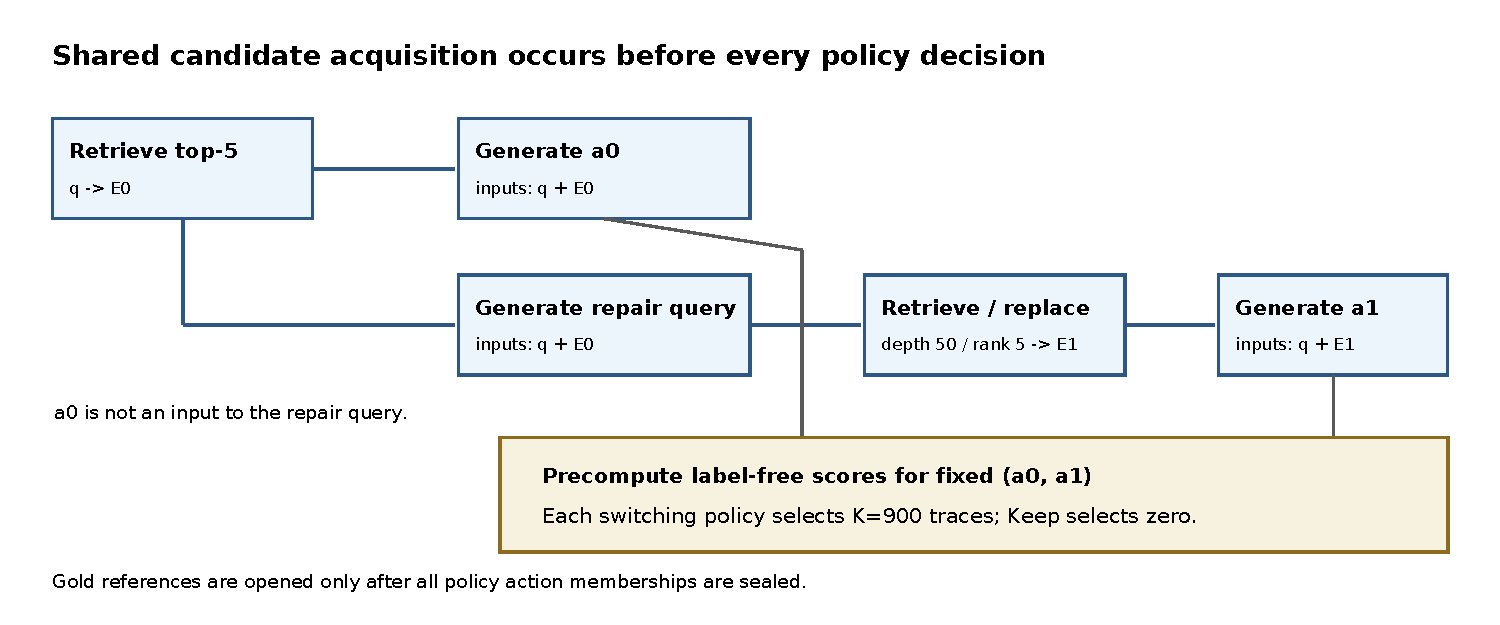
\includegraphics[width=\linewidth]{figures/paired_pipeline.pdf}
\caption{Shared paired candidate acquisition and downstream fixed-batch selection. Retrieval, repair-query generation, and both answers are acquired before policy allocation. Gold references are opened only after action memberships are sealed.}
\label{fig:pipeline}
\end{figure}

\subsection{Scores and policies}
The shared label-free score matrix contains 11 numeric inputs. Seven are outputs of byte-fixed historical upstream estimators: state-symmetric HGB, state-symmetric logistic, no-cross-state, no-$B$, no-evidence-change, no-answer-form, and ordinary compact logistic. Three are fixed rules: $B$-rule, higher-own-likelihood, and likelihood margin. The eleventh is the paired GbV margin.

For the paired adaptation of GbV Post-Answering NLI, the verifier assigns the maximum entailment probability over evidence chunks for each branch, $F_0(a_0,E_0)$ and $F_1(a_1,E_1)$; the policy input is $F_1-F_0$. The verifier is MoritzLaurer/deberta-v3-large-zeroshot-v2.0 at revision \nolinkurl{5a4338ab2151dc8db04ad53b42b6153382bf4f99}, evaluated in FP32 with 512 tokens, 20-word chunk overlap, and entailment label index zero. The branch difference, revision/runtime, eligibility mask, and global allocation are project choices, not an author-supplied paired-policy formula or author-code reproduction. Base scoring also uses BGE answer-pair embeddings and four Qwen teacher-forced likelihood cells. These computations precede evaluation-outcome access.

The full panel contains Keep; raw HGB; raw paired GbV; ROA-FULL; ROA-NOGBV; HGB+\allowbreak GbV$_R$; HGB-\allowbreak only$_R$; GbV-\allowbreak only$_R$; and a sealed historical V2 policy. The subscript $R$ denotes a fitted Recovery head. The five fitted policies are supervision matched:
\begin{itemize}
  \item ROA-FULL uses all 11 numeric inputs, 11 missingness flags, and three retriever indicators (25 columns);
  \item ROA-NOGBV removes the GbV input and flag (23 columns);
  \item HGB+GbV$_R$ uses HGB and the paired GbV margin, their missingness flags, and retriever indicators (7 columns);
  \item HGB-only$_R$ and GbV-only$_R$ each use one score, one missingness flag, and retriever indicators (5 columns).
\end{itemize}
Raw HGB, raw GbV, and V2 have different upstream training or rule dependencies and serve as context rather than matched attribution controls. HGB is an upstream score and comparator. HGB+GbV$_R$ is ordinary calibrated logistic regression.

\subsection{Matched supervision and allocation}
All five heads use the same 4,500 development questions and 13,500 traces. Within each dataset, deterministic hash order assigns 1,200 questions to fitting and 300 disjoint questions to calibration; retriever siblings stay together. Fit-only medians, means, and population standard deviations are used for preprocessing. Missingness and retriever indicators are unscaled.

The binary target is Recovery, defined by normalized EM changing from incorrect for $a_0$ to correct for $a_1$. This target does not directly optimize Net or impose a Damage constraint; Damage reduction is an evaluated outcome. Each base head is L2 logistic regression with $C=1$, \texttt{lbfgs}, no class weights, \texttt{max\_iter}=5000, and tolerance $10^{-4}$. A separate Platt logistic model with $C=10^6$, \texttt{lbfgs}, \texttt{max\_iter}=2000, and tolerance $10^{-4}$ calibrates disjoint calibration-set logits. The five base/calibration bundles account for ten of 185 total scientific fits in the complete project history; no model was refit after fresh outcomes were observed.

The fresh evaluation retains all 18,000 traces. A common eligibility mask contains 4,267 traces. The 13,732 traces with equal normalized answers and one trace with an empty original answer are forced to Keep for every policy. Every switching policy ranks eligible traces by its frozen score and receives the same global allocation $K=\operatorname{round}(0.05\times18{,}000)=900$. Ties use \texttt{(dataset,retriever,sample\_id)}. There are no dataset quotas, retriever quotas, tuned thresholds, or post-outcome action changes.

\subsection{Gold firewall, outcomes, and inference}
For the evaluation cohort, candidate acquisition, all scores, the eligibility mask, and complete action memberships were sealed before reference access. A separate mapper then evaluated 6,000 selected reference sets (6,863 strings) against 36,000 fixed answers and emitted numeric EM/F1 outcomes only. An independent method-blind implementation recomputed all 72,000 scalars. This establishes the documented order within the authenticated execution graph, not the absence of unknown activity outside that graph.

For a policy action, Recovery is $a_0$ incorrect and $a_1$ correct; Damage is $a_0$ correct and $a_1$ incorrect; Neutral contains the other two transitions and need not mean unchanged token F1. Net equals Recovery minus Damage. EM and token F1 use the full 18,000-trace denominator. Damage rate is $100\times\damage/18{,}000$ percent, and the EM difference from Keep is $100\times(\recovery-\damage)/18{,}000$ percentage points.

The primary family contains three ordered comparisons and two endpoints per comparison: EM difference and Damage-rate difference. We use 20,000 dataset-stratified question-cluster bootstrap draws with NumPy \texttt{default\_rng(20260926)}, keeping all retriever siblings together and reallocating the global top-$K$ actions in each draw. Percentile endpoints use quantiles $0.05/12$ and $1-0.05/12$ with linear interpolation, applying a two-sided Bonferroni adjustment to the six-endpoint family. The joint rule passes only when the adjusted EM range is strictly above zero and the adjusted Damage range is strictly below zero. A secondary sensitivity analysis reuses the draws while holding observed action memberships fixed; it does not enforce exactly 900 action copies within each draw. Intervals condition on the fitted heads and realized candidate pools. They exclude uncertainty from model fitting, calibration, candidate generation, and pool construction, and do not provide exact finite-sample coverage or guarantees for new readers or domains.

\section{Results}
\subsection{Complete policy panel}
Table~\ref{tab:all-results} reports every policy. Keep has an EM of 17.9889\% and token F1 of 22.7207\%. Each switching policy executes 900 actions. Their EM gains over Keep range from 1.6278 to 1.9389 percentage points, while their Damage rates range from 0.0611\% to 0.2111\%. All eight comparisons with Keep are descriptive and are outside the frozen primary interval family.

HGB+GbV$_R$ records 352 Recoveries and 11 Damages (Net 341), yielding 19.8833\% EM and 25.2780\% token F1. Among the eight equal-action switching policies it has the lowest observed full-population Damage count and rate. Keep, which takes no actions, has zero Damage. ROA-FULL has the highest point EM and F1, but its 371 Recoveries are accompanied by 22 Damages; point ranking alone does not establish advancement.

\begin{table*}[t]
\centering
\caption{Complete fixed-allocation results. EM, F1, and Damage rate are percentages; $\Delta$EM and $\Delta$F1 are differences from Keep in percentage points. Actions, Recovery, Damage count, Neutral, and Net are trace-event counts. All rates use 18,000 traces. Keep takes no action.}
\label{tab:all-results}
\resizebox{\textwidth}{!}{% Generated from sealed POINT_ESTIMATES.json; do not edit by hand.
\begin{tabular}{lrrrrrrrrrr}
\toprule
Policy & Act. & Rec. & Dmg. & Neu. & Net & EM (\%) & $\Delta$EM (pp) & F1 (\%) & $\Delta$F1 (pp) & Dmg. rate (\%) \\
\midrule
Keep & 0 & 0 & 0 & 0 & +0 & 17.9889 & +0.0000 & 22.7207 & +0.0000 & 0.0000 \\
HGB & 900 & 366 & 32 & 502 & +334 & 19.8444 & +1.8556 & 25.1593 & +2.4386 & 0.1778 \\
GbV & 900 & 318 & 25 & 557 & +293 & 19.6167 & +1.6278 & 24.8928 & +2.1722 & 0.1389 \\
ROA-FULL & 900 & 371 & 22 & 507 & +349 & 19.9278 & +1.9389 & 25.2988 & +2.5781 & 0.1222 \\
ROA-NOGBV & 900 & 355 & 38 & 507 & +317 & 19.7500 & +1.7611 & 25.0321 & +2.3115 & 0.2111 \\
HGB+GbV$_R$ & 900 & 352 & 11 & 537 & +341 & 19.8833 & +1.8944 & 25.2780 & +2.5574 & 0.0611 \\
HGB-only$_R$ & 900 & 357 & 26 & 517 & +331 & 19.8278 & +1.8389 & 25.1323 & +2.4117 & 0.1444 \\
GbV-only$_R$ & 900 & 323 & 24 & 553 & +299 & 19.6500 & +1.6611 & 24.9344 & +2.2137 & 0.1333 \\
V2 & 900 & 361 & 28 & 511 & +333 & 19.8389 & +1.8500 & 25.1712 & +2.4506 & 0.1556 \\
\bottomrule
\end{tabular}
}
\end{table*}

\begin{figure}[t]
\centering
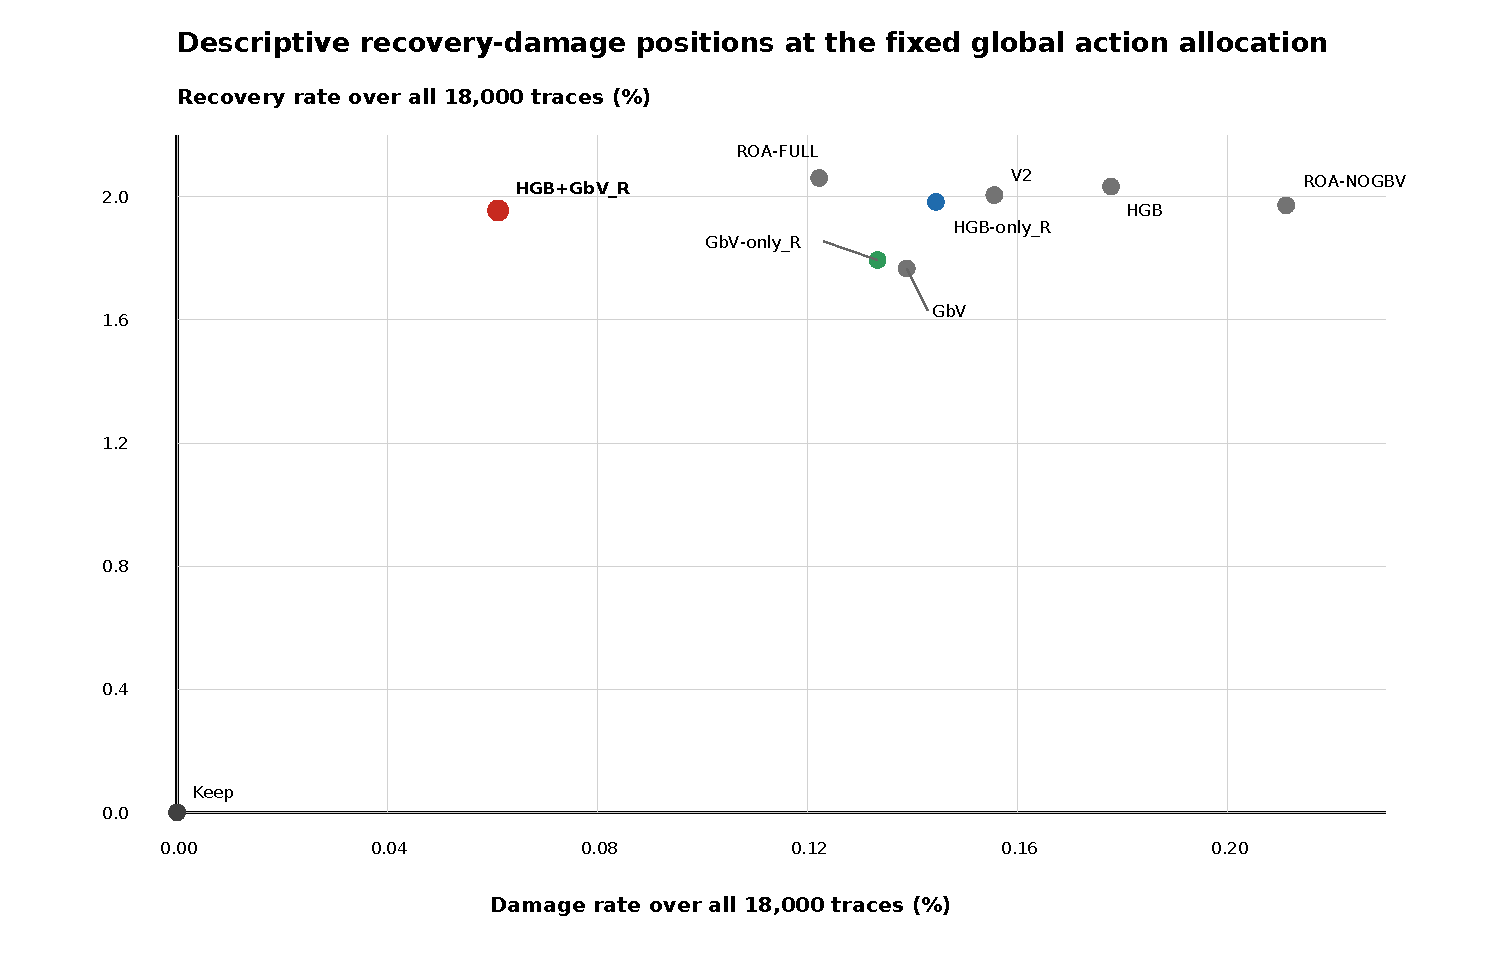
\includegraphics[width=\linewidth]{figures/recovery_damage.pdf}
\caption{Descriptive full-population Recovery and Damage rates. The chart contains no uncertainty intervals; formal inference is restricted to Table~\ref{tab:primary}.}
\label{fig:recovery-damage}
\end{figure}

\subsection{Primary comparisons}
Table~\ref{tab:primary} gives the complete primary family. Relative to GbV-only$_R$, HGB+GbV$_R$ improves EM by 0.2333 percentage points and reduces Damage by 0.0722 points. The adjusted ranges, [0.0722, 0.4333] and [-0.1444, -0.0278], exclude zero in the required directions, so this comparison passes the joint rule. In event counts, the difference is 42 more correct final answers and 13 fewer Damage events across 18,000 traces.

Relative to HGB-only$_R$, HGB+GbV$_R$ changes EM by 0.0556 points with an adjusted range of [-0.1556, 0.3167]. Its Damage difference is -0.0833 points with range [-0.1833, -0.0056]. Because the EM range crosses zero, the joint rule does not pass. This comparison cannot support a claim that adding GbV to HGB jointly improves accuracy and harm.

ROA-FULL minus HGB+GbV$_R$ is 0.0444 points for EM [-0.1333, 0.2037] and +0.0611 points for Damage [0.0000, 0.1278]. It also fails the joint rule, and the Damage direction is not favorable. The 25-feature model therefore does not establish an advance over the simpler two-signal policy.

\begin{table*}[t]
\centering
\caption{Primary ordered comparisons. Ranges are multiplicity-adjusted percentiles from 20,000 dataset-stratified question-cluster bootstrap draws with top-$K$ actions reallocated in each draw. All values are percentage points.}
\label{tab:primary}
\resizebox{\textwidth}{!}{% Primary, top-$K$ reallocated within each bootstrap draw; generated from sealed INTERVALS.json.
\begin{tabular}{lrrrrl}
\toprule
Ordered comparison & $\Delta$EM & Adjusted range & $\Delta$Damage & Adjusted range & Joint rule \\
\midrule
ROA-FULL $-$ HGB+GbV$_R$ & +0.0444 & [-0.1333, +0.2037] & +0.0611 & [+0.0000, +0.1278] & Not met \\
HGB+GbV$_R$ $-$ HGB-only$_R$ & +0.0556 & [-0.1556, +0.3167] & -0.0833 & [-0.1833, -0.0056] & Not met \\
HGB+GbV$_R$ $-$ GbV-only$_R$ & +0.2333 & [+0.0722, +0.4333] & -0.0722 & [-0.1444, -0.0278] & Met \\
\bottomrule
\end{tabular}
}
\end{table*}

The primary comparisons test different increments. The positive comparison adds HGB to a GbV-only head; the inconclusive comparison adds GbV to an HGB-only head. One passing and one non-passing comparison is not a formal interaction test or evidence that the increments differ causally. It also does not imply that GbV is unnecessary: the study was not designed as an equivalence or non-inferiority test.

\subsection{Sensitivity and secondary breakdowns}
Holding the observed action memberships fixed preserves the HGB+GbV$_R$ versus GbV-only$_R$ joint decision: adjusted EM and Damage ranges are [0.0389, 0.4278] and [-0.1389, -0.0222]. The HGB-only comparison remains non-passing: its EM range crosses zero and its Damage upper endpoint touches zero. The ROA-FULL comparison also remains non-passing. Dataset and retriever breakdowns are reported in the supplement as descriptive consequences of the one global allocation. They were not separate primary families, and no favorable subgroup is promoted to a claim.

\section{Workload and reproducibility evidence}
All policies consume the same precomputed graph in this experiment. Candidate acquisition executes 18,000 original and 18,000 repair retrievals. Original retrieval comprises 12,000 BM25 and 12,000 dense components, 15,422 embedding forwards, and 54,716 document rows. Repair retrieval comprises 12,000 BGE query forwards without document re-embedding. The Qwen stage contains 54,000 generation receipts, 51,901,556 prompt tokens, and 826,362 generated tokens/output score steps. Base scoring records 2,250 answer-embedding and 16,932 likelihood forwards, with 136 likelihood cache hits; paired GbV records 8,534 NLI forwards over 42,946 premise/hypothesis pairs.

Preserved stage timers are 1,096.562 s for C2, 45,216.887 s for C3, 5,337.573 s for base scoring, 3,523.022 s for GbV scoring, and 157.658 s for fixed allocation. Their boundaries include different setup, caching, I/O, and audit work, so they are not summed or presented as end-to-end latency. Saved C4 allocator peaks are 8,153,970,176 bytes for base scoring and 2,956,706,304 bytes for GbV scoring; they occurred in different stages and are not additive.

No standalone policy deployment was built or timed. Canonical C2/C3 allocator peaks, per-trace latency distributions, one end-to-end timer, energy, and FLOPs were not measured. Consequently, the global 5\% action count is not a claim of 5\% retrieval, generation, latency, memory, or compute.

The numerical analysis is backed by hash-pinned aggregate files and independent implementations. A deterministic anonymous aggregate package contains the complete point estimates, intervals, claim summary, code/data availability statement, and verification scripts. Its current candidate archive hash is \nolinkurl{b785890366995c2943007f5635e622814bc7961dc7b3ded4adee0707dfb7ca8d}. Public distribution is withheld until a project license and target-journal policy are selected.

\section{Threats to validity}
\paragraph{Reader and population scope.}
The accepted result uses one 3B-parameter Qwen reader, three multi-hop QA datasets, three fixed retrieval conditions, and bounded benchmark-derived pools. This scale does not invalidate the within-reader matched comparison, but it prevents claims about reader size, other model families, unseen domains, full-corpus retrieval, or production use. A Phi extension produced authentic runtime artifacts but failed its prospectively fixed semantic validation gate; it supplies no effect result. A planned Mistral extension stopped before engineering and model execution.

\paragraph{Candidate and estimand scope.}
The repair operation replaces only rank 5 after a generated repair query. Other repair operators can change candidate quality and policy ranking. The estimand conditions on both candidates already existing, the fixed eligibility mask, and a global 900-action allocation. It does not measure an online threshold policy or compute-aware router.

\paragraph{Metric scope.}
Normalized EM is strict and can miss semantically correct variants; token F1 is included descriptively. Recovery and Damage measure correctness transitions rather than evidence faithfulness. The GbV component remains a paired adaptation of a faithfulness verifier. Damage uses the full population denominator, so its numerical rate should be interpreted with the event count and action count.

\paragraph{Inference scope.}
Question-cluster resampling respects retriever siblings and stratifies datasets, but the intervals condition on fixed fitted heads and realized pools. The study does not independently replicate the candidate-generation population. Secondary dataset/retriever cells are small, correlated views of the same global action allocation.

\paragraph{Provenance and contamination.}
The selected cohort has no dataset/ID overlap with a known 18,600-question exclusion union, but ID separation is not semantic decontamination and cannot rule out model pretraining exposure or unknown unlogged historical use. Benchmark-supplied contexts may also share dataset-specific structure with answers despite the field-restricted pool construction. Seven historical upstream estimators are byte-fixed and their saved-parameter computation is replayed, yet their original per-estimator fit-time ID/matrix receipts, an independent original-fit witness, and an independently recovered earlier pin of the complete historical training manifest are missing. Later receipts do not reconstruct that absent evidence. Reproduction therefore authenticates the saved computation within checked environments, not a literal replay of every original training event. The supplement records the distinct historical and current development populations.

\section{Discussion}
The main result is comparison dependent. Starting from a GbV-only fitted selector, adding the internal HGB score is supported by both endpoints. Starting from HGB-only, the available data do not establish that adding GbV jointly improves EM and Damage. This pattern can arise from redundancy, score quality, finite event counts, calibration, or the realized candidate set. The experiment does not distinguish these mechanisms.

The result also illustrates why unmatched comparisons can mislead. Raw scores and historical V2 do not share the same development recipe as the five fitted controls. Comparing the two-signal head only with raw GbV would mix feature value with supervision and calibration. Likewise, selecting ROA-FULL from the highest point EM would ignore uncertainty and its less favorable observed Damage. Matched single-signal heads isolate a more precise question even when the answer is negative.

For deployment, the study supports neither a universal fusion rule nor a cost saving. All candidates and scores were precomputed for fairness. A real system would need a prospectively timed standalone graph, an online allocation or threshold rule, drift monitoring, and validation on its own reader and corpus. Those engineering decisions are outside the present evidence.

\section{Conclusion}
On a fixed 6,000-question Qwen2.5-3B-Instruct cohort with three datasets, three retrievers, shared original/repaired candidates, matched supervision, and a global 5\% action allocation, the HGB+\allowbreak GbV$_R$ selector improves EM and reduces Damage relative to GbV-\allowbreak only$_R$. The same joint rule does not pass against HGB-\allowbreak only$_R$, and a larger feature stack does not advance over the two-signal selector. The contribution is the controlled attribution and its negative boundary, together with full-population harm accounting. It is not a new selector architecture or evidence of transfer beyond the evaluated reader and candidate pipeline.

\section*{Data availability}
An anonymous, aggregate-only verification package has been built and independently validated. It contains no questions, answers, Gold strings, per-example outcomes, model weights, local paths, or identities. Public distribution remains pending owner selection of a project license and the final journal's data/code policy. Canonical private artifacts and immutable hashes can support confidential review subject to those policies. The manuscript does not claim end-to-end public reproducibility before these gates close.

\section*{Declarations}
Author identities, affiliations, contributions, funding, competing interests, institutional ethics wording, acknowledgements, and any required disclosure of writing assistance are maintained in the separate title-page/declarations template and must be completed by the responsible authors before submission.

\bibliographystyle{plainnat}
\bibliography{references}
\end{document}
